\chapter{Results and Discussion}

The data and discussion of results below come in a combination of data gathered using the OONI probe in Ireland and Iraq, as well as published OONI data from the OONI Measurement Aggregation Toolkit (MAT).

\section{Test Results}

\subsection{Website Accessibility Results}

\subsubsection{Collected Data}

The first part of this section is an analysis of the data collected by the OONI probe locally in Ireland and through the VM in Iraq.

The results below are an average of the number of websites blocked each day over the testing period of 9 days.

\begin{table}[H]
\centering
\caption{Summary of Blocked vs. Unblocked Websites by Country}
\begin{tabular}{lcc}
\toprule
\textbf{Country} & \textbf{Unblocked} & \textbf{Blocked} \\
\midrule
Ireland & 105 & 32 \\
Iraq    & 108 & 29 \\   
\bottomrule
\end{tabular}
\label{tab:blocked_summary}
\end{table}

Table 4.2 shows the distribution of blocking methods in Ireland and Iraq.

\begin{table}[H]
\centering
\caption{Distribution of Blocking Methods Detected in Iraq and Ireland}
\begin{tabular}{lcc}
\toprule
\textbf{Blocking Method} & \textbf{Iraq Frequency} & \textbf{Ireland Frequency} \\
\midrule
TCP/IP         & 18 & 15 \\
DNS            & 1  & 6  \\
HTTP           & 3  & 1  \\
Error/Failure  & 8  & 5  \\
\bottomrule
\end{tabular}
\label{tab:blocking_methods_comparison}
\end{table}

The table below shows the number of websites blocked in each category in both countries.

\begin{table}[H]
\centering
\caption{Blocked Websites by Category and Country}
\begin{tabular}{lccc}
\toprule
\textbf{Category} & \textbf{Total Websites Tested} & \textbf{Ireland} & \textbf{Iraq} \\
\midrule
Uncategorized                      & 30 & 12 & 10 \\
Piracy / Streaming / File Sharing  & 20 & 10 & 4 \\
News / Media                       & 20 & 2 & 2 \\
Adult Content                      & 20 & 0 & 0 \\
Creative / Educational / Misc      & 15 & 0 & 0 \\
General / National Services        & 9 & 1 & 2 \\
Streaming / Social Media           & 9 & 1 & 1 \\
Religious                          & 4 & 2 & 3 \\
VoIP / Communication               & 2 & 1 & 1 \\
Gambling                           & 2 & 2 & 2 \\
Email/Privacy Tools                & 2 & 0 & 1 \\
Adult / Alcohol                    & 2 & 0 & 2 \\
LGBTQ+                             & 1 & 1 & 1 \\
AI / Technology                    & 1 & 0 & 0 \\
\bottomrule
\end{tabular}
\label{tab:category_block}
\end{table}

\subsubsection{Public OONI Data}

This section is an analysis of publicly available OONI data over the previous 30 day period in Ireland and Iraq. The data in table 4.5 is the average over the 30-day period.

\begin{table}[H]
\centering
\caption{Website Blocking based on Public OONI Data}
\begin{tabular}{lcc}
\toprule
\textbf{} & \textbf{Ireland} & \textbf{Iraq} \\
\midrule
Number of Websites Tested           & 1695 & 3703 \\
Number of Successful Connections    & 1628 & 3353 \\
Number of Anomalies                 & 43 & 262 \\
Number of Failures                  & 24 & 88 \\
\bottomrule
Percentage of Total Blocked         & 2.5\% & 7\% \\
\end{tabular}
\label{tab:category_block}
\end{table}

\begin{figure}[H]
    \centering
    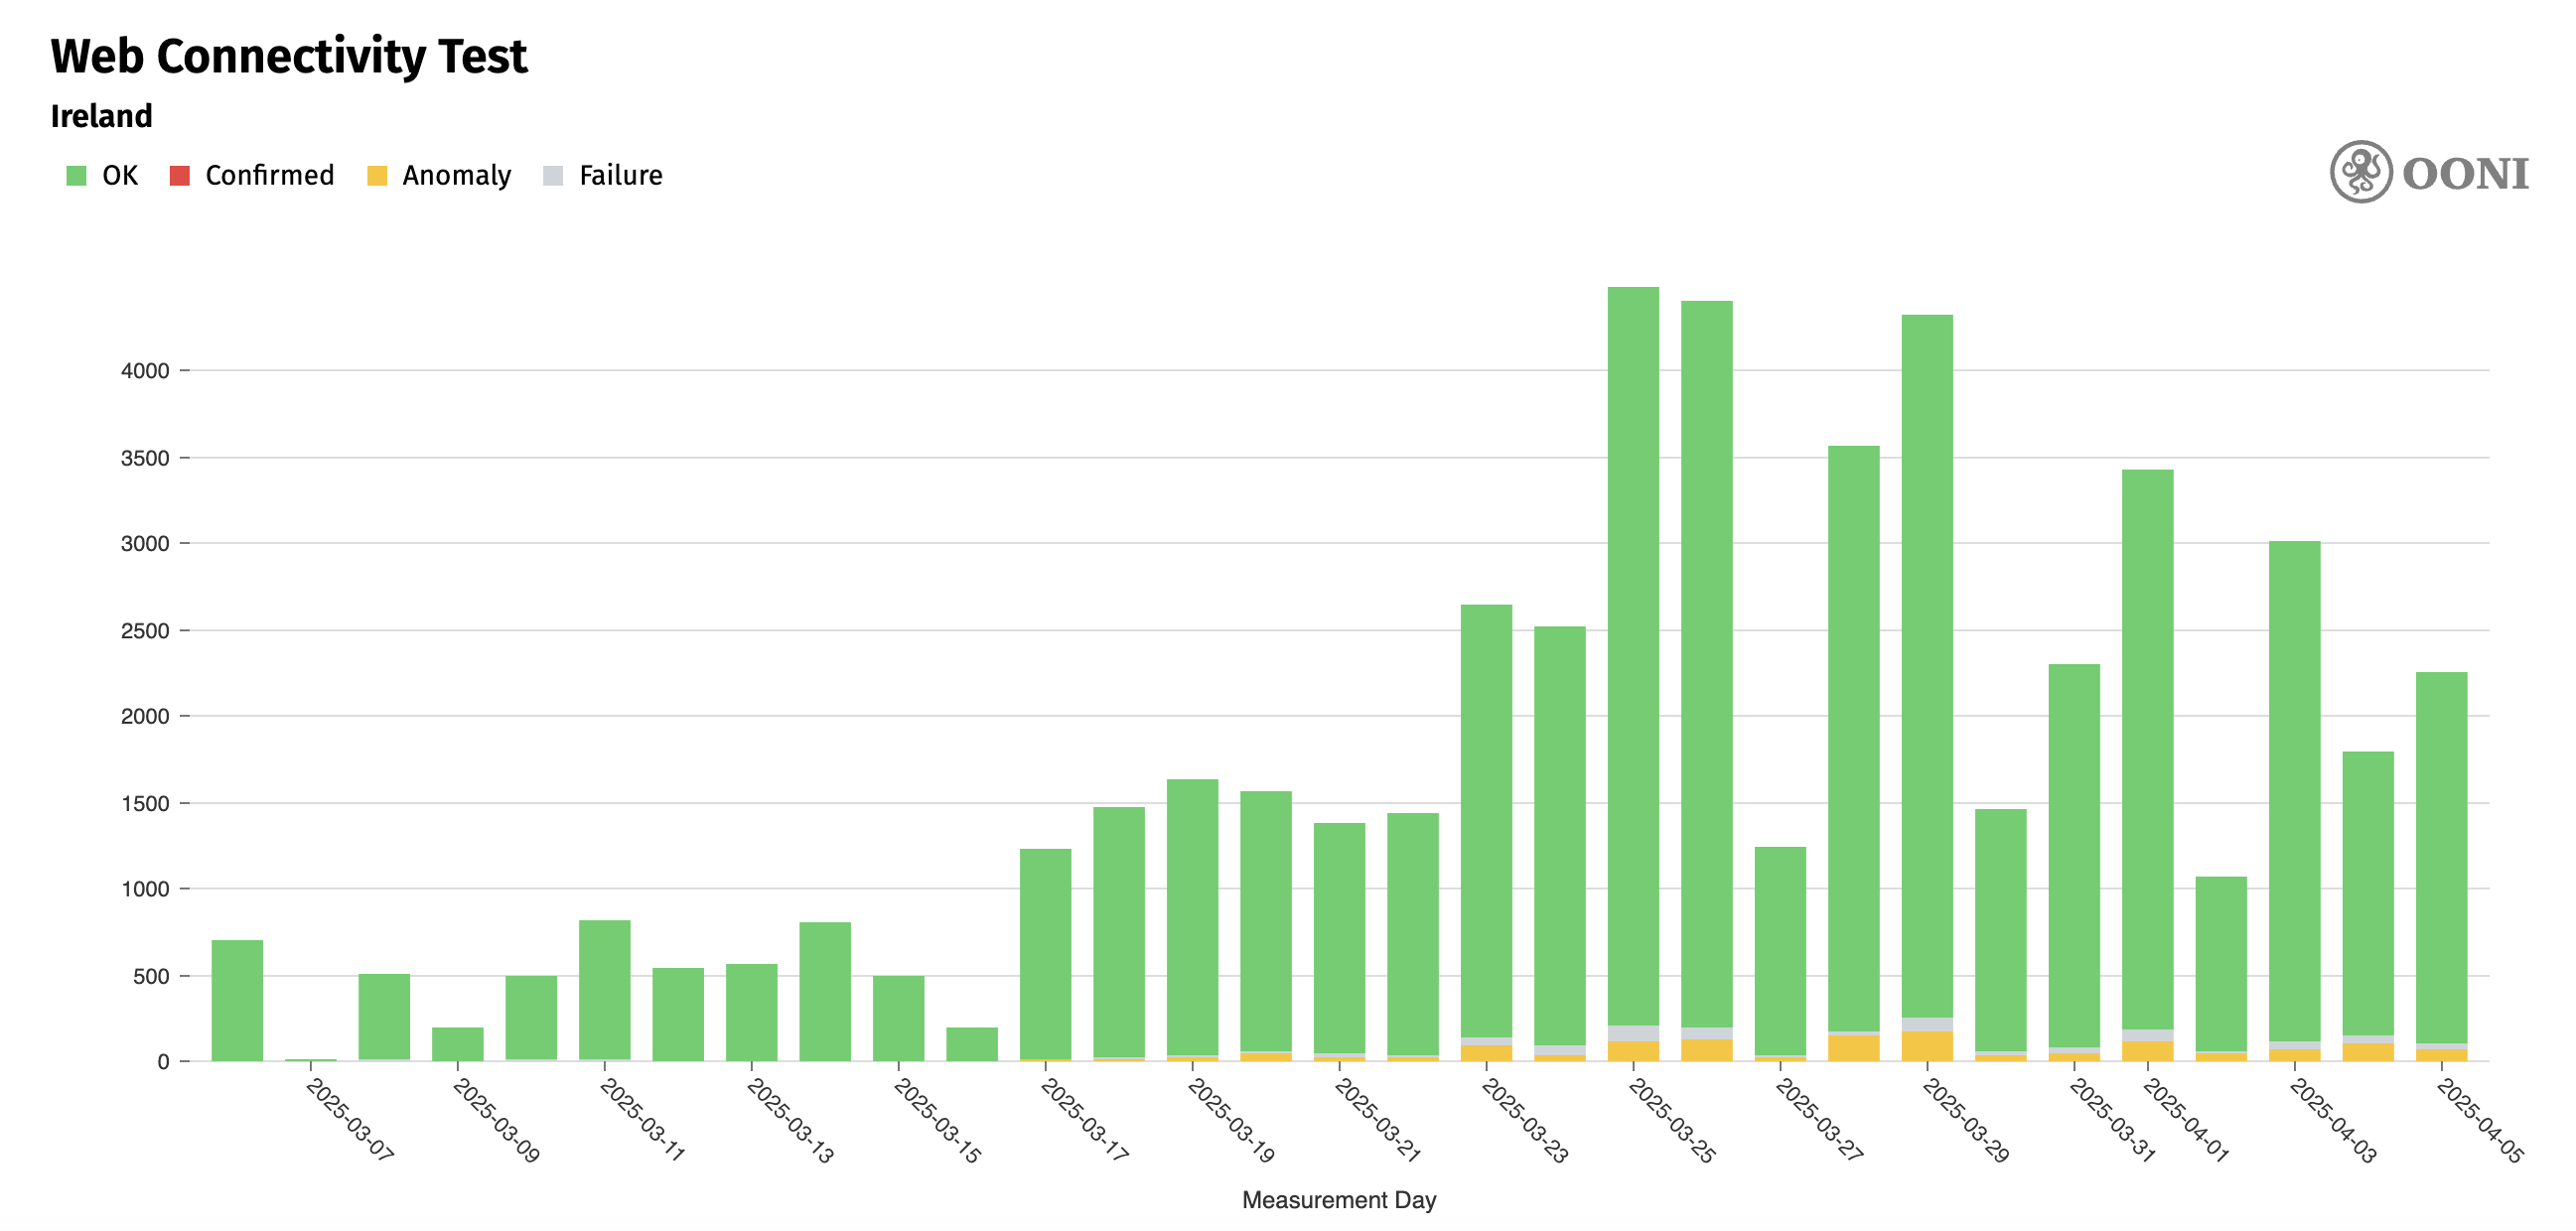
\includegraphics[width=\textwidth]{Griff/TCD SCSS CAPSTONE/Results/IrelandWebsiteTest.png}
    \caption{Ireland Web Connectivity Test: March 6, 2025 -- April 6, 2025}
    \label{fig:iraq-middlebox-HTTP-manipulation}
\end{figure}

\begin{figure}[H]
    \centering
    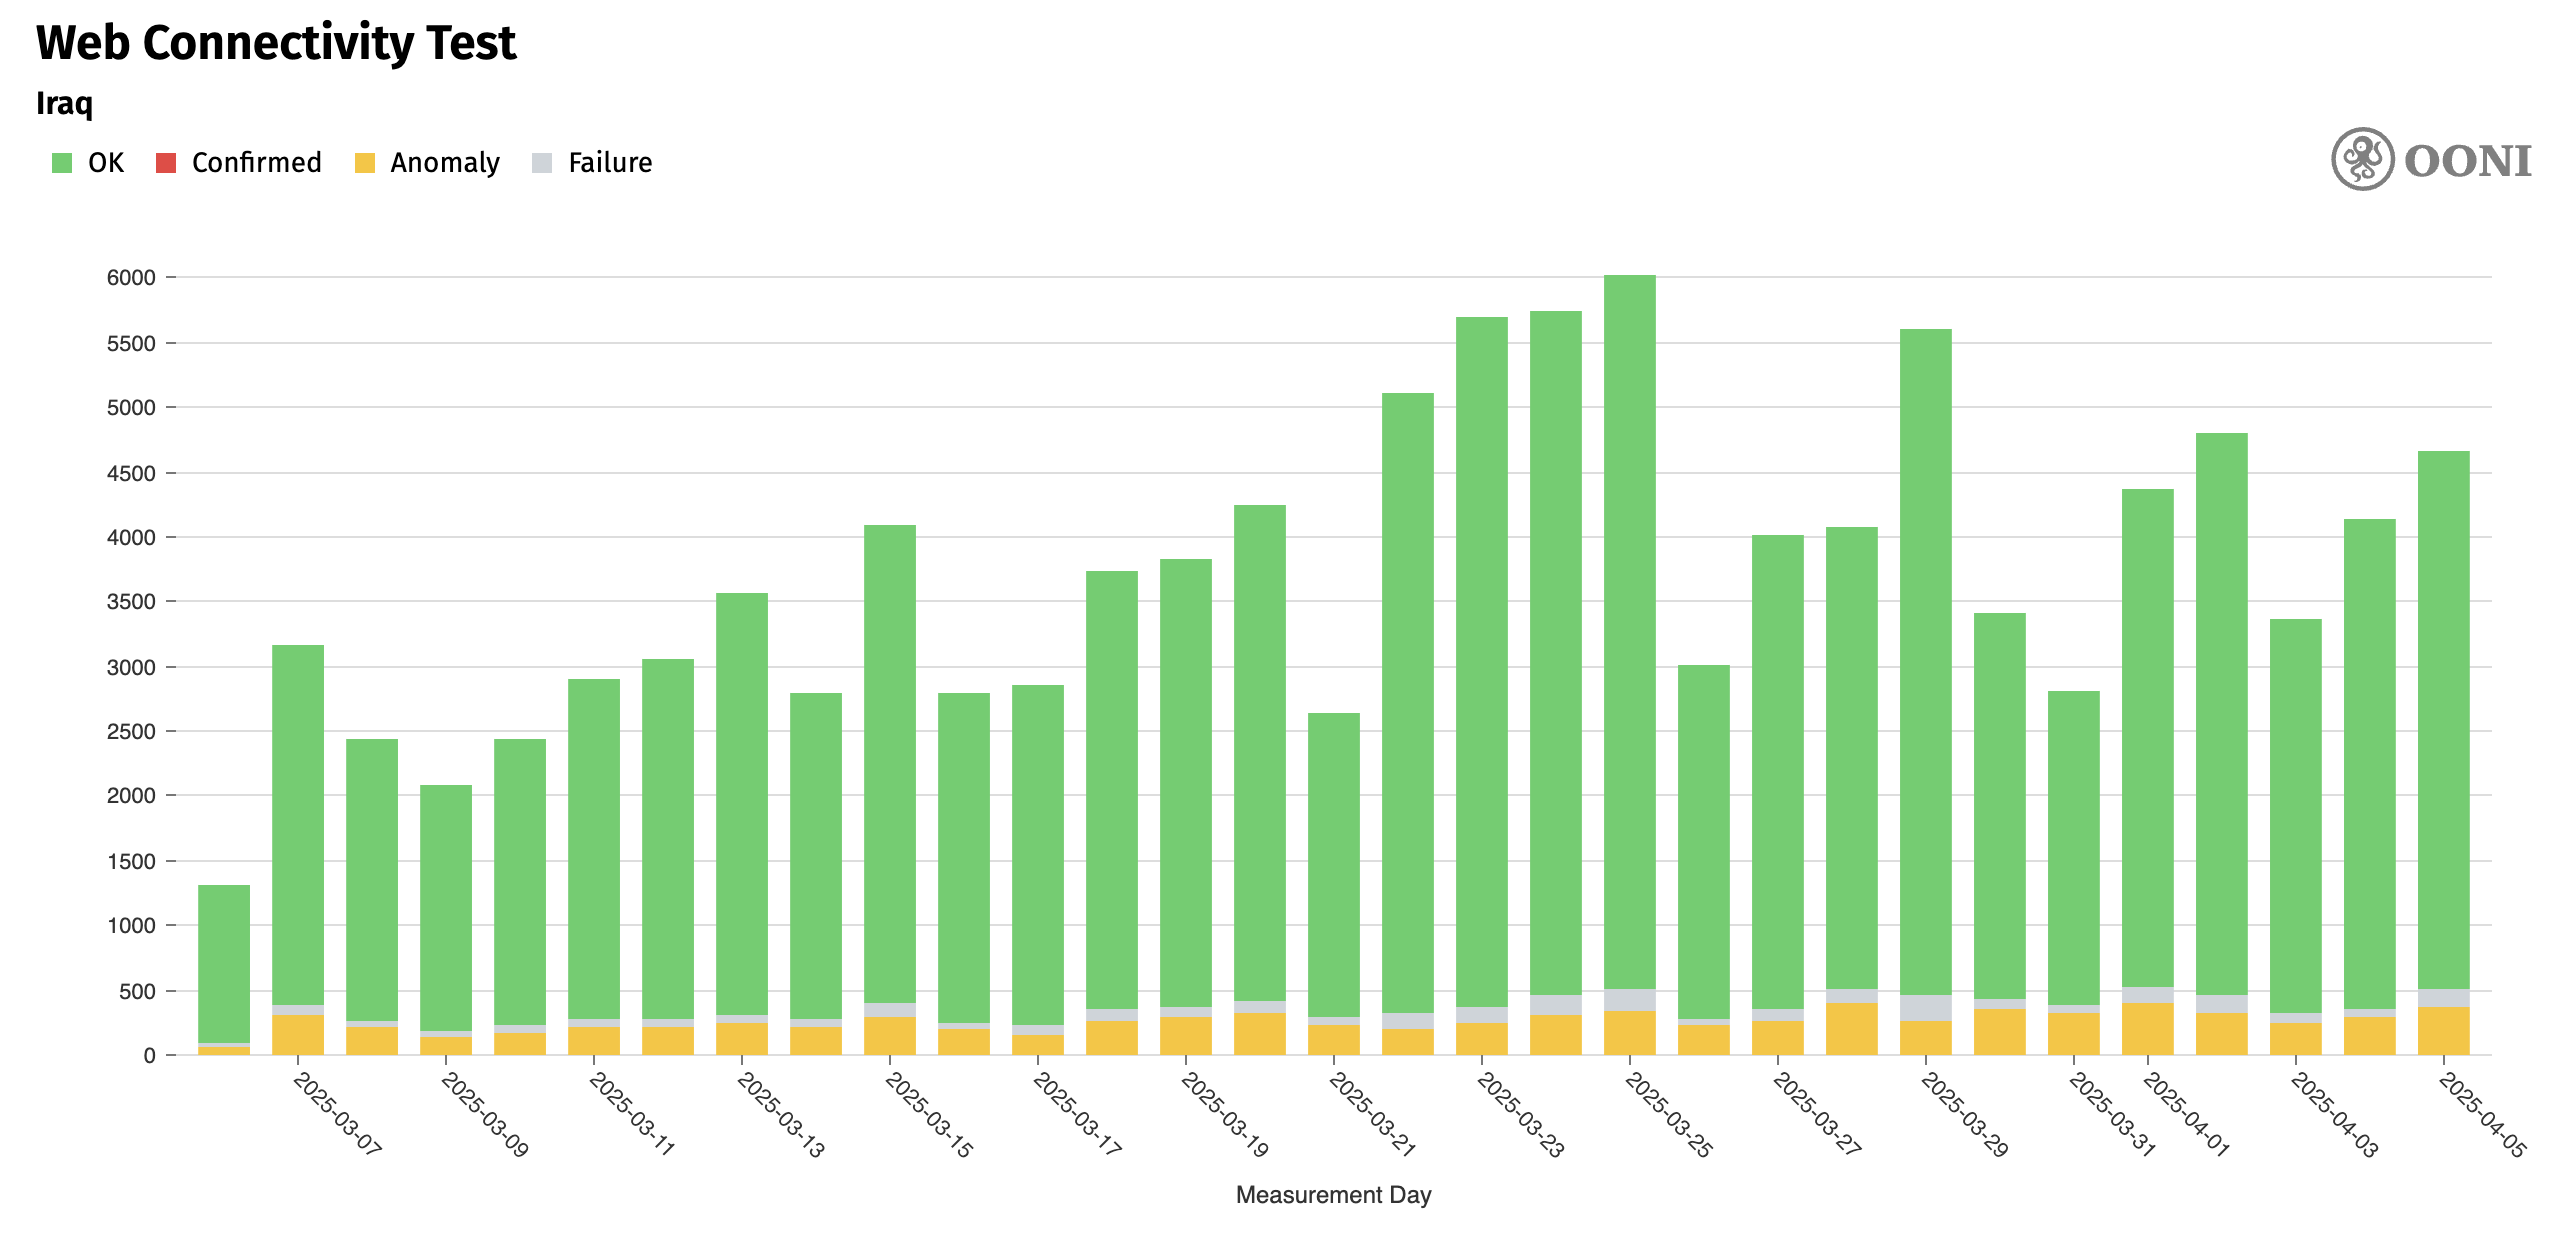
\includegraphics[width=\textwidth]{Griff/TCD SCSS CAPSTONE/Results/IraqWebsiteTest.png}
    \caption{Iraq Web Connectivity Test: March 6, 2025 -- April 6, 2025}
    \label{fig:iraq-middlebox-HTTP-manipulation}
\end{figure}

\subsection{Circumvention Test Results}

\subsubsection{Ireland}

Ireland likely does not block Tor on any of its ASNs, as it is largely accessible outside of 2 anomalies.

\textbf{March 18, 2025} - Magnet Networks Limited (AS34245) - Tor Test (1 anomaly out of 78 measurements)
%https://explorer.ooni.org/m/20250318181530.182975_IE_tor_8b558463294b2881

\textbf{March 31, 2025} - Liberty Global B.V. (AS6830) - Tor Test (1 anomaly out of 191 measurements)
%https://explorer.ooni.org/m/20250331102020.562562_IE_tor_913ee551111fe0a9

Outside of these two anomalies, there is no evidence that Tor is being blocked in Ireland.

Psiphon on the other hand yielded different results. While Psiphon was largely able to be accessed on most ASNs, there were a few where access is likely blocked. 

\begin{table}[H]
\centering
\caption{ASN's with Evidence of Psiphon being Blocked in Ireland}
\begin{tabular}{lccc}
\toprule
\textbf{ASN} & \textbf{Anomaly} & \textbf{Total Measurement Count} & \textbf{Percentage} \\
\midrule
AS1213    & 33 & 35  & 94\% \\
AS6830    & 16 & 215 & 7.4\% \\
AS8075    & 1  & 1   & 100\% \\
AS13280   & 8  & 12  & 66\% \\
AS15751   & 1  & 9   & 11\% \\
\bottomrule
Totals    & 60 & 494 & 12.1\% \\
\end{tabular}
\label{tab:category_block}
\end{table}

\subsubsection{Iraq}

Similar to Ireland, Iraq largely does not block access to Tor outside of a few outliers.

\textbf{March 20, 2025} - Super Cell Network for Internet Services LTD (AS209193) - Tor Test (1 anomaly out of 92 measurements)
%https://explorer.ooni.org/m/20250320220102.873661_IQ_tor_3796e6aaa913670d

\textbf{March 30, 2025} - Hulum Almustakbal Company for Communication Engineering and Services Ltd (AS203214) - Tor Test (2 anomalies out of 160 measurements)
%https://explorer.ooni.org/m/20250330191838.341920_IQ_tor_f0e7ccd345c39d7f

\textbf{March 30, 2025} - Valin Company for General Trading and Communications LTD (AS205254) - Tor Test (1 anomaly out of 17 measurements)
%https://explorer.ooni.org/m/20250330111106.914884_IQ_tor_f45745fcedc21407

Outside of these anomalies, there is no significant evidence that Tor is being blocked in Iraq.

There is also little evidence of Psiphon being blocked in Iraq at a significant scale. Aside of a few outliers, Psiphon only seemed to be blocked on one ASN. 

\begin{table}[H]
\centering
\caption{ASN's with Evidence of Psiphon being Blocked in Iraq}
\begin{tabular}{lccc}
\toprule
\textbf{ASN} & \textbf{Anomaly} & \textbf{Total Measurement Count} & \textbf{Percentage} \\
\midrule
AS203214  & 127 & 165  & 77\% \\
AS51684   & 4   & 23   & 17\% \\
AS199739  & 1   & 352  & 0.2\% \\
AS205254  & 1   & 30   & 3.3\% \\
AS208324  & 1   & 3    & 33\% \\
\bottomrule
Totals    & 134 & 1107 & 12.1\% \\
\end{tabular}
\label{tab:category_block}
\end{table}

Based on this data, Psiphon is widely accessible in Iraq outside of AS203214.

\subsection{Instant Messaging Test Results}

The results of the Instant Messaging tests were very similar in Ireland and Iraq. Both tests showed no signs of interference or blocking of Facebook Messenger, Telegram, Whatsapp, or Signal. However, looking outside of the tested ASNs reveals a significant difference between the two countries. The tested data in Ireand is consistent with public OONI data, and shows no blocking of instant messaging platforms. The Iraq data is also consistent with tests run on the same ASN, but in Iraq there are other ASNs that show signs of blocking.

\subsubsection{Ireland}

In the past 30-day period, there were only 2 anomalies found that shows any kind of instant messaging blocking:

\textbf{March 24, 2025} - Packethub S.A. (AS136787) - Facebook Messenger Test (1 anomaly out of 3 measurements)
%https://explorer.ooni.org/m/20250324111124.418686_IE_facebookmessenger_fbdc8895400acaba

\textbf{March 24, 2025} - HEAnetCLG (AS1213) - Signal Test (1 anomaly out of 37 measurements)
%https://explorer.ooni.org/m/20250324164458.153631_IE_signal_667f7ad13e55043a

Outside of these anomalies, there was no evidence of instant messaging blocking.

\subsubsection{Iraq}

Iraq had significant evidence of instant messaging platforms being blocked in certain ASNs. The table below shows each ASN, and the percentage of tests where there was an anomaly found.

\begin{table}[H]
\centering
\caption{ASN's with Evidence of Instant Message Platform Blocking in Iraq}
\begin{tabular}{lcccc}
\toprule
\textbf{ASN} & \textbf{Facebook} & \textbf{Telegram} & \textbf{WhatsApp} & \textbf{Signal} \\
\midrule
AS203214  & 27\%  & 7.8\% & 25\%  & 44\% \\
AS205254  & 26\%  & 3.8\% & 7.6\% & 7.6\% \\
AS199739  & 1\%   & 0.5\% & 0.2\% & 0.8\% \\
AS13335   & 47\%  & 0\%   & 0\%   & 0\% \\
AS50710   & 33\%  & 0\%   & 0\%   & 0\% \\
AS206206  & 60\%  & 0\%   & 0\%   & 0\% \\
AS212330  & 100\% & 0\%   & 0\%   & 0\% \\
AS210022  & 0\%   & 0\%   & 0\%   & 82\% \\
AS51020   & 0\%   & 0\%   & 0\%   & 32\% \\
AS202651  & 0\%   & 0\%   & 0\%   & 23\% \\
AS59588   & 0\%   & 0\%   & 1.9\% & 1.9\% \\
AS209193  & 0\%   & 0\%   & 0.7\% & 0\% \\
\bottomrule
Total Percentage Blocked  & 6.2\%   & 1.4\%   & 4.1\% & 6.2\% \\
\end{tabular}
\label{tab:category_block}
\end{table}

Instant Messaging platforms are essentially widely available in Iraq, but there are some areas where blocking does occur.

\subsection{Middlebox Test Results}

The results of the Middlebox Test were the same for both countries. Both the HTTP Header Field Manipulation and HTTP Invalid Request Line tests resulted in no Middleboxes being detected in either country. However, while there was no evidence of Middleboxes being found using the providers tested, it is possible that other providers in both countries have Middleboxes present in the network.

Using publicly available OONI data for Ireland and Iraq, it was found that there were cases of Middleboxes being detected in both countries over the past 30 days (March 6, 2025 - April 6, 2025). 

\subsubsection{Ireland}

There is very little evidence of Middleboxes being present in Ireland. Over the past 30-day period, there are only two anomalies present. Both of these anomalies are from the HTTP Invalid Request Line test. 

\textbf{March 25, 2025} - Meteor Mobile Communications Ireland (AS15751) (1 anomaly out of 9 measurements)
%https://explorer.ooni.org/m/20250325122211.663367_IE_httpinvalidrequestline_c713442d98eebb5c

\textbf{April 1, 2025} - Vodafone Ireland Limited (AS15502) (1 anomaly out of 79 measurements)
%https://explorer.ooni.org/m/20250401215651.365763_IE_httpinvalidrequestline_51f20fe7e9d31698

These results are likely outliers, as there are very little Middlebox tests for Meteor Mobile Communications Ireland in this time span and no other anomalies for Vodafone Ireland Limited.

\subsubsection{Iraq}

There is considerably more evidence of Middleboxes being present in Iraq. Over the past 30 day period, there were 125 anomalies in the HTTP Invalid request line Test and 19 anomalies in the HTTP Header Field Manipulation Test.

The table below lists the ASNs that were suspected to have Middleboxes present using the HTTP Invalid Request Line test. It then shows the number of anomalies, the total measurement count, and what percentage of the total count were anomalies. Note that any ASN that had less than 0.5\% anomalies was ignored.

\begin{table}[H]
\centering
\caption{ASN's with Evidence of Middleboxes (HTTP Invalid Request Line Test) in Iraq}
\begin{tabular}{lccc}
\toprule
\textbf{ASN} & \textbf{Anomaly} & \textbf{Total Measurement Count} & \textbf{Percentage} \\
\midrule
AS198589  & 68 & 70 & 97\% \\
AS203214  & 32 & 158 & 20.25\% \\
AS59588   & 13 & 53 & 24.5\% \\
AS13335   & 8 & 10 & 80\% \\
AS48492   & 2 & 4 & 50\% \\
AS50710   & 1 & 1 & 100\% \\
\bottomrule
Total Percentage   & 125 & 1071 & 11.6\% \\
\end{tabular}
\label{tab:category_block}
\end{table}

%\begin{figure}[H]
%    \centering
%    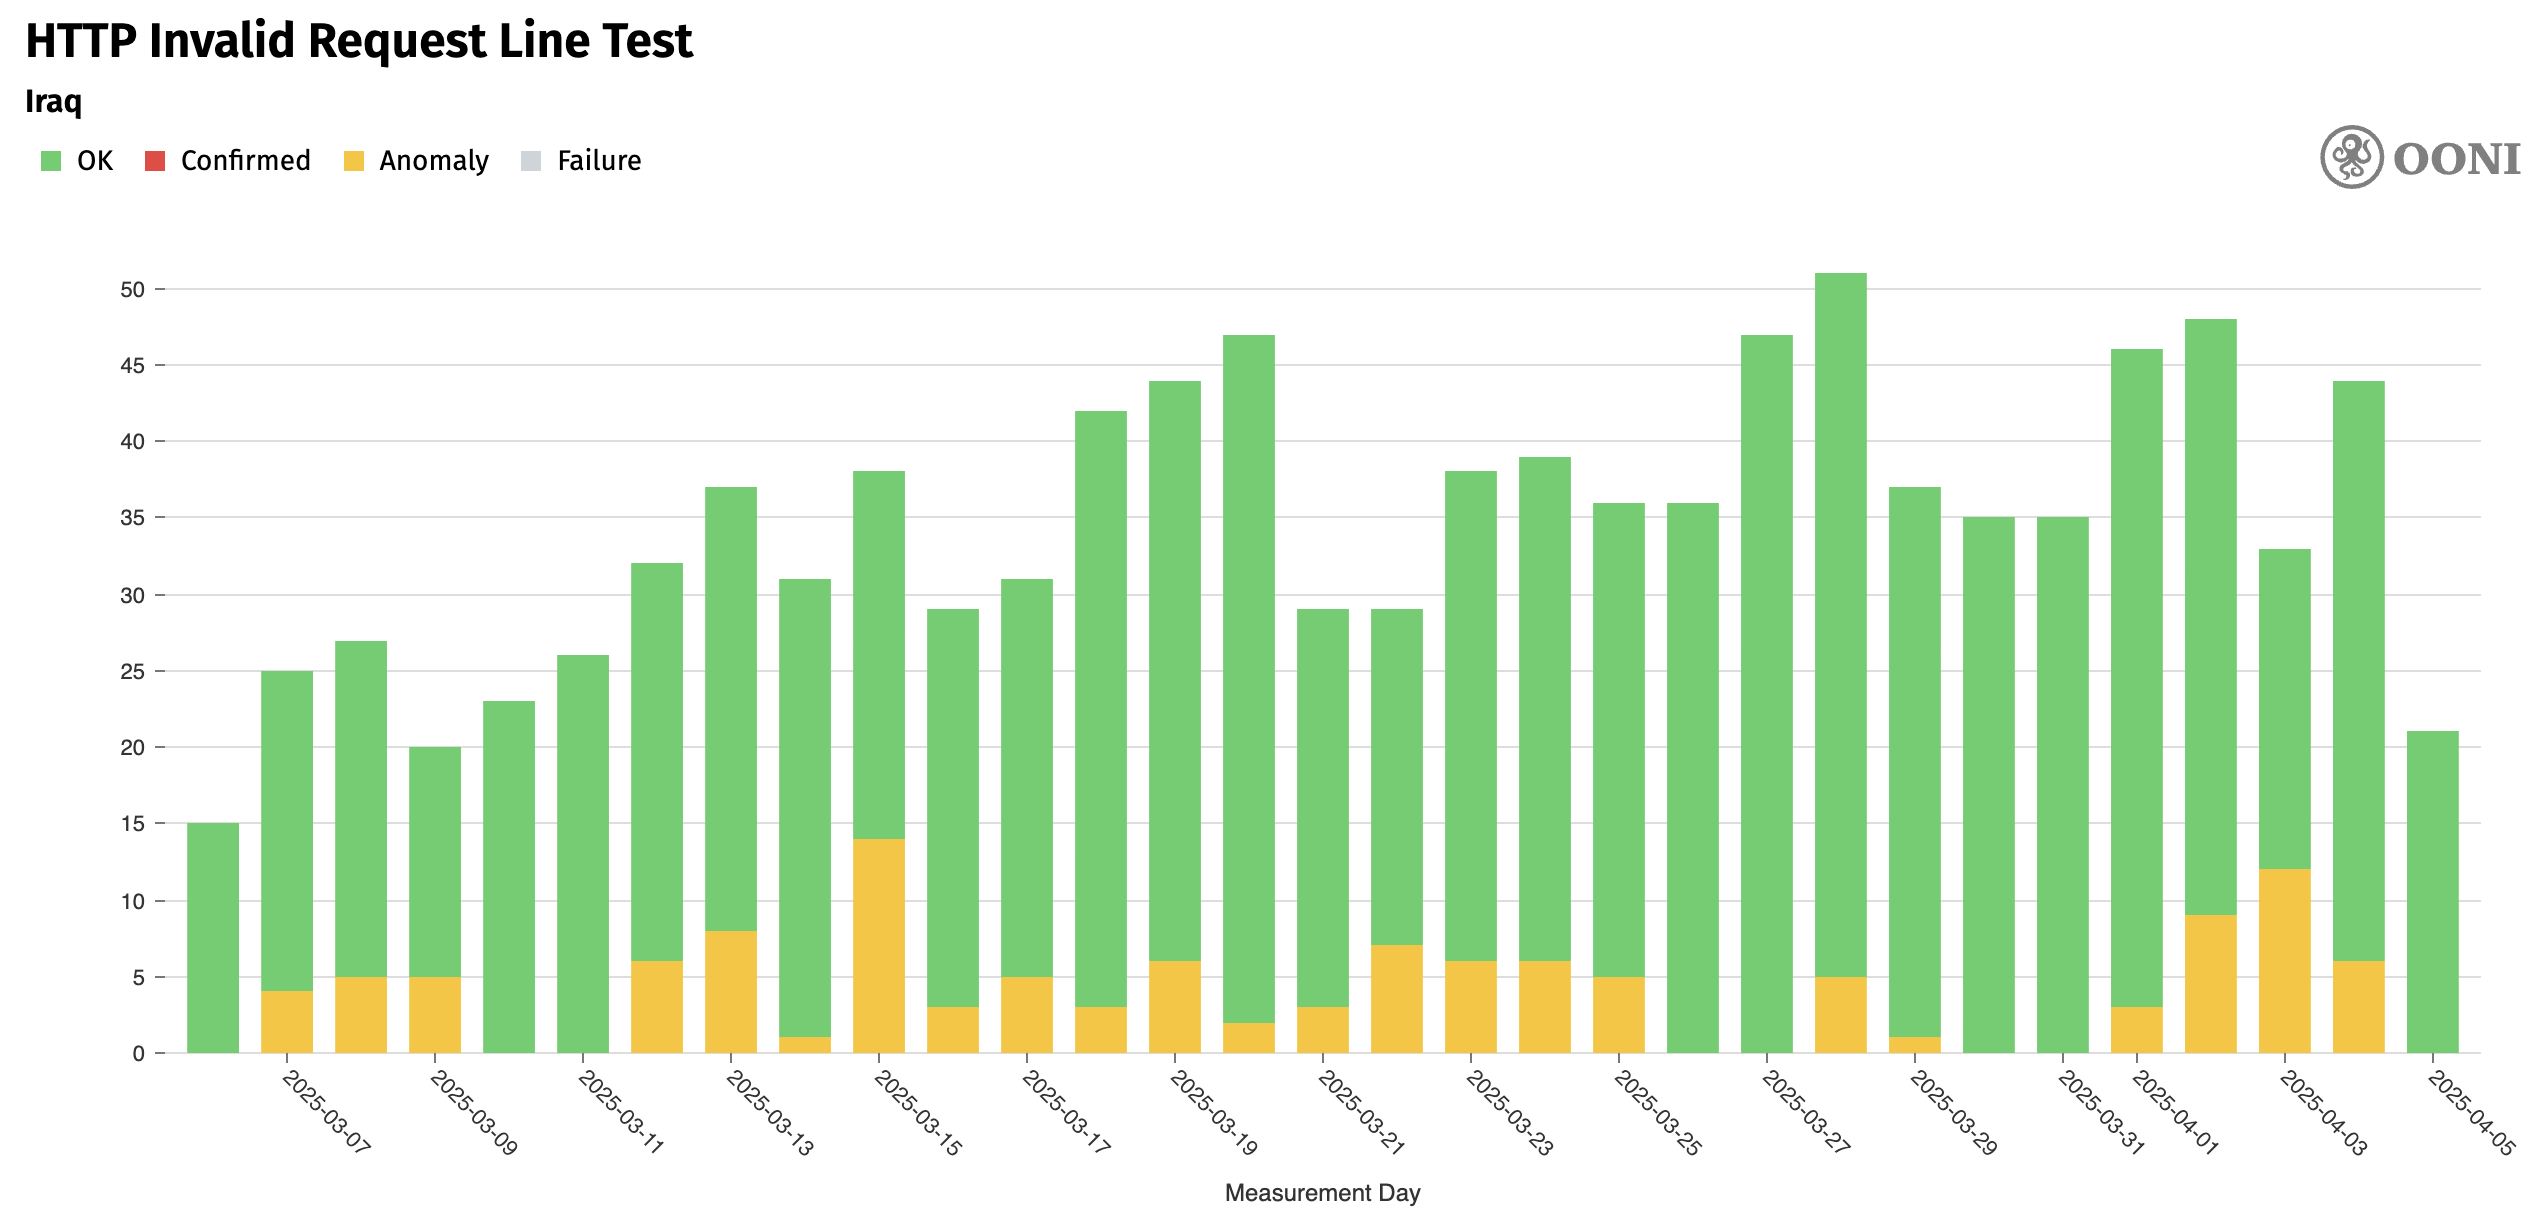
\includegraphics[width=\textwidth]{Griff/TCD SCSS CAPSTONE/Results/IraqMiddleboxHTTPInvalidTest.png}
 %   \caption{Iraq Middlebox HTTP Invalid Request Line Test: March 6, 2025 -- April 6, 2025}
%    \label{fig:iraq-middlebox-invalid-request}
%\end{figure}

The table below lists the ASNs that were suspected to have Middleboxes present using the HTTP Header Field Manipulation test. It then shows the number of anomalies, the total measurement count, and what percentage of the total count were anomalies. Note that any ASN that had less than 0.5\% anomalies was ignored.

\begin{table}[H]
\centering
\caption{ASN's with Evidence of Middleboxes (HTTP Header Field Manipulation Test) in Iraq}
\begin{tabular}{lccc}
\toprule
\textbf{ASN} & \textbf{Anomaly} & \textbf{Total Measurement Count} & \textbf{Percentage} \\
\midrule
AS13335   & 8 & 10 & 80\% \\
AS48492   & 2 & 4 & 50\% \\
AS50710   & 1 & 1 & 100\% \\
\bottomrule
Total Percentage   & 19 & 1074 & 1.7\% \\
\end{tabular}
\label{tab:category_block}
\end{table}


%\begin{figure}[H]
 %   \centering
%    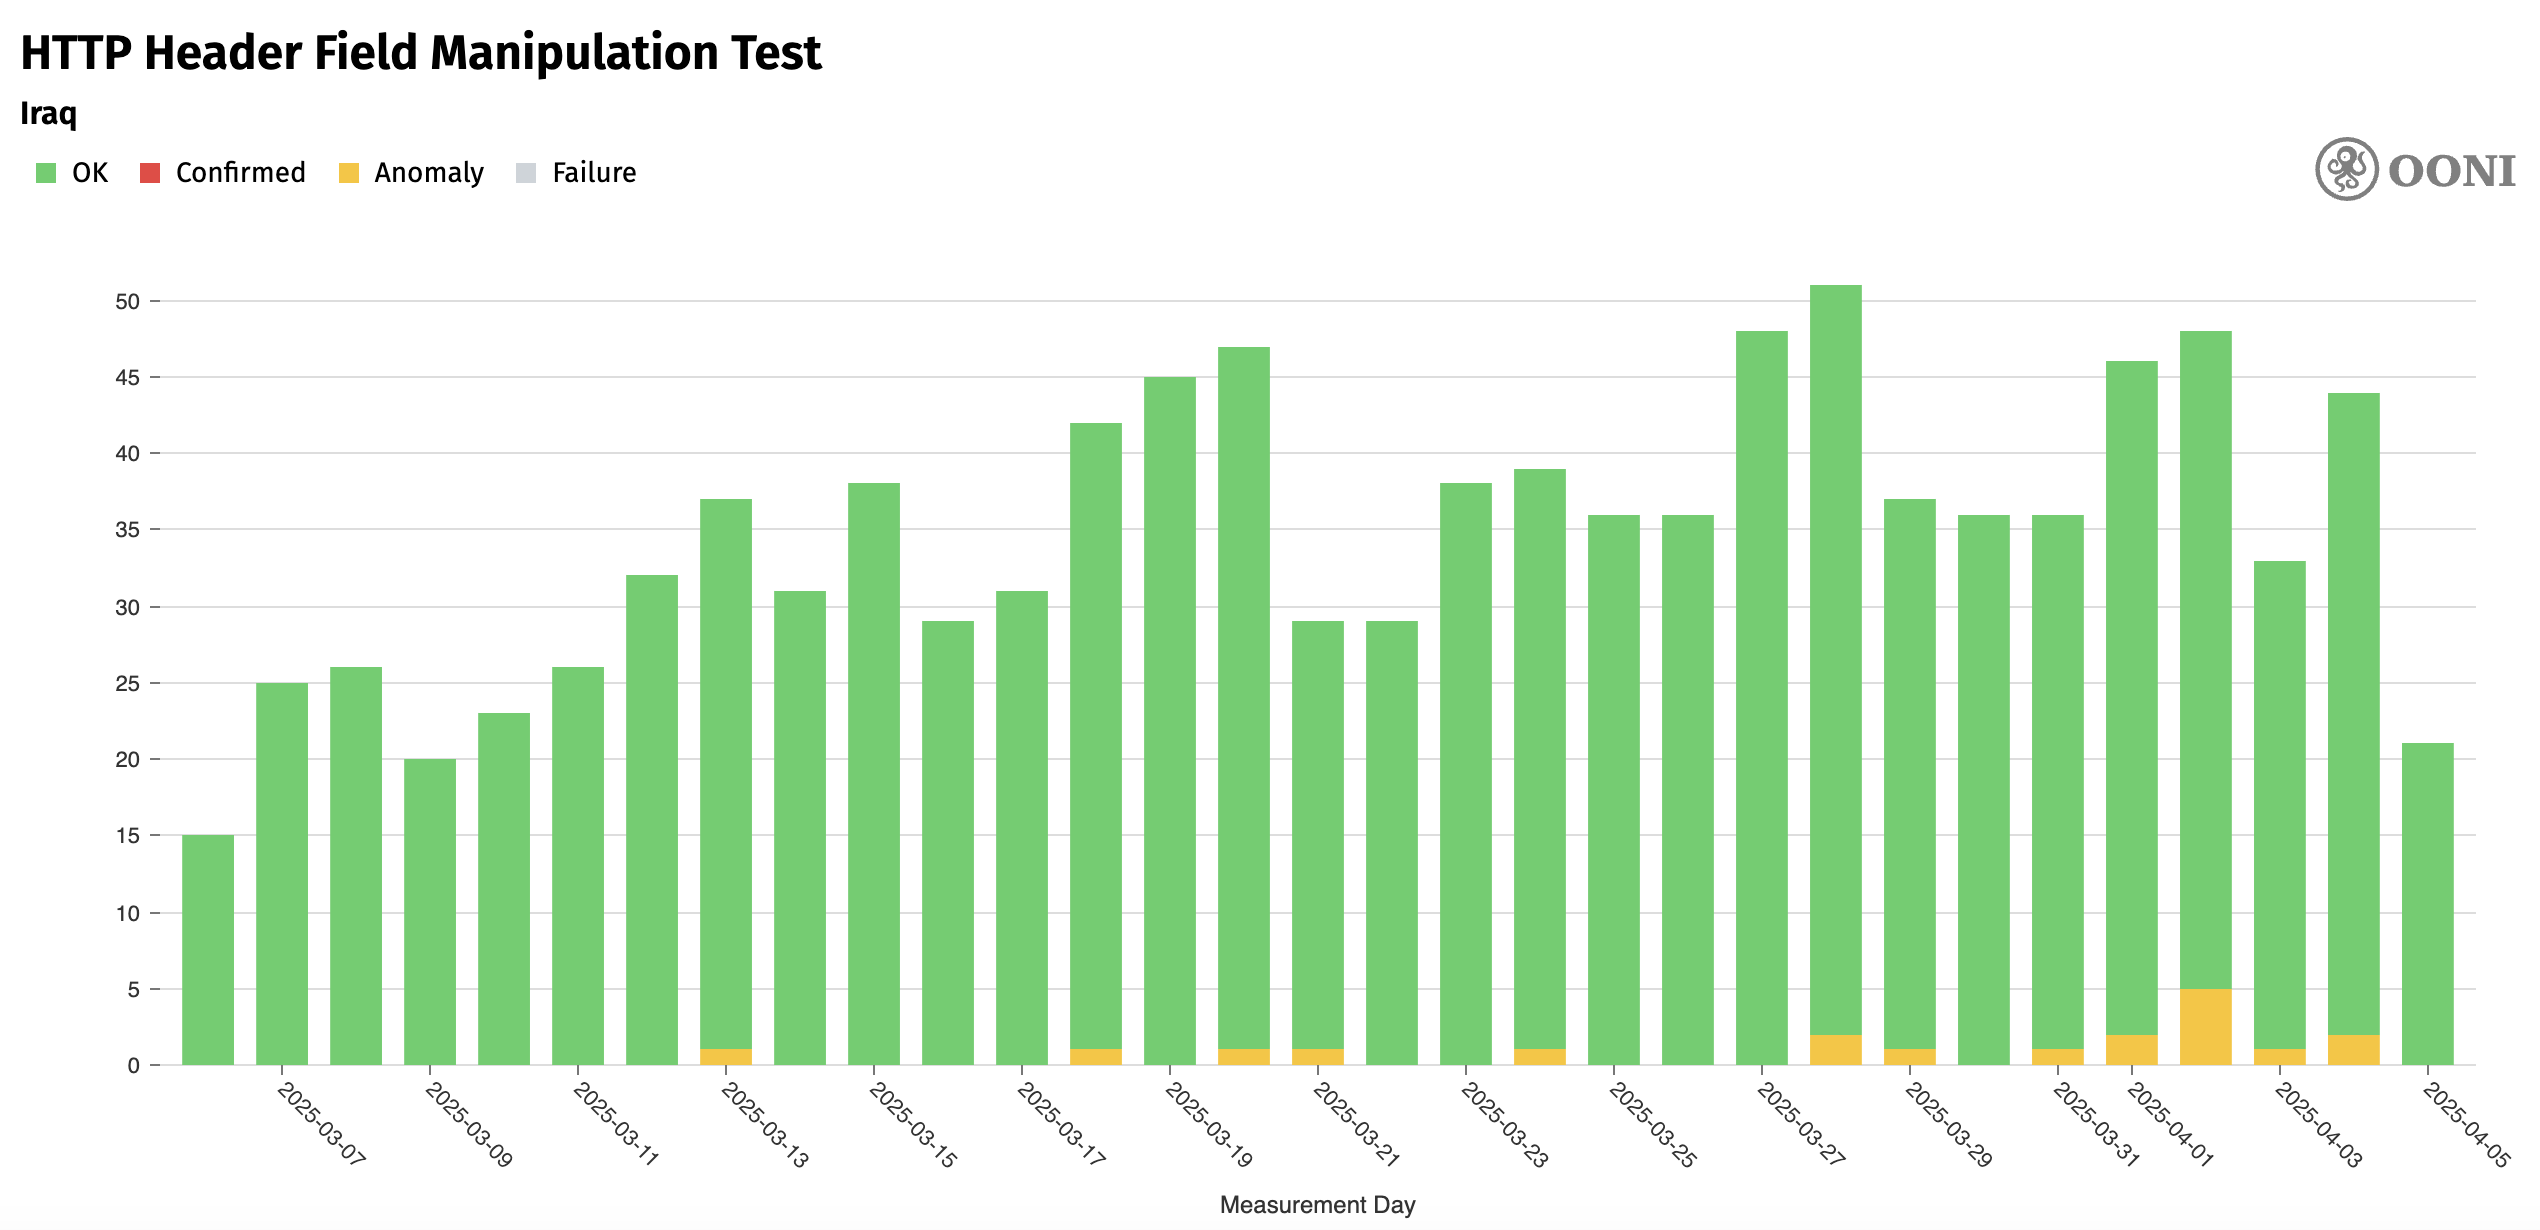
\includegraphics[width=\textwidth]{Griff/TCD SCSS CAPSTONE/Results/IraqMiddleboxHTTPManipulation.png}
%    \caption{Iraq Middlebox HTTP Header Field Manipulation Test: March 6, 2025 -- April 6, 2025}
%    \label{fig:iraq-middlebox-HTTP-manipulation}
%\end{figure}

\textit{Note: All CSV files gathered from the public OONI database can be found on the public GitHub for this work; see Appendix A1.2.}


\section{Comparative Analysis: Ireland v. Iraq}

The combined results of OONI probe testing and public OONI data reveal differences in censorship between Ireland and Iraq. While both countries implement content restrictions and other blocks, there are significant differences in the scale and motivations behind these blocks.

\subsubsection{Website Accessability}

(waiting on some final data from OONI)

\subsubsection{Circumvention Tools}

The accessibility of Tor and Psiphon were largely the same in Ireland and Iraq outside of a few exceptions. Tor was widely accessible in both countries, indicating that both Ireland and Iraq have no significant mechanisms in place to block this tool, and if they do there is no evidence that it is effective. There is evidence that Psiphon is blocked on specific ASNs in both countries, with public OONI data backing this up. Over the same 30-day period, both Ireland and Iraq blocked Psiphon 12.1\% of the time. As a result, there is little evidence that there are systemic efforts to block access to Psiphon, similar to Tor.

\subsubsection{Instant Messaging Platforms}

In Ireland, there is essentially no evidence that instant messaging services are blocked in any meaningful manner. This is inline with Ireland's stance on censorship, and was expected. In Iraq however, there is some evidence that instant messaging services are blocked in some areas, but according to public OONI data they are widely accessible. There are ASNs that had implemented blocks on all four services tested to some capacity, which can indication regional blocking in response to certain events. This is aligned with Iraq's more reactionary censoring practice.

\subsubsection{Presence of Middleboxes}

The use of Middleboxes was almost non-existant, as there were only two anomalies over the 30-day time period, which were likely false-positives. This data indicates that Ireland does not implement TLS or SNI-based filtering in any systematic or widespread manner. By contrast, Iraq showed significant evidence of Middleboxes being present. AS198589 showed significant signs of Middleboxes being present, and there are other ASNs with significant anomalies. This indicates that Iraq may implmelent TLS or SNI-based filtering in some areas of the country, which makes sense as we know that much of Iraq's current censorship efforts are decentralized. 

\subsection{Summary of Comparative Observations}

\begin{table}[H]
\centering
\caption{Comparative Summary of Internet Censorship: Ireland vs. Iraq}
\begin{tabular}{lcc}
\toprule
\textbf{Metric} & \textbf{Ireland} & \textbf{Iraq} \\
\midrule
Block Rate (OONI) & 2.5\% & 7\% \\
Blocking Methods & -- & -- \\
Tool Blocking & Rare, selective & Targeted, ASN-specific \\
Messaging Blocking & Negligible & Present on some ASNs \\
Middleboxes Detected & Minimal & Present on some ASNs \\
Motivations & Legal, EU compliance & Political, cultural control \\
\bottomrule
\end{tabular}
\label{tab:comparison_summary}
\end{table}

These findings support the initial research, showing that Ireland and Iraq have quite different approaches to censorship. Ireland maintains a limited, legal-centric censorship model, which is transparent and aligned with most other Western nations. Iraq's approach, while less centralized, is more reactive and inconsistent, with it often being tied to internal events. 

